% IMPORTANT: PLEASE USE XeLaTeX FOR TYPESETTING
\documentclass{sintefbeamer}
\usepackage{xeCJK}
\usepackage{amsthm}
\setbeamertemplate{theorems}[numbered]
\makeatletter
\setbeamertemplate{footline}
{
  \leavevmode%
  \hbox{%
  \begin{beamercolorbox}[wd=.7\paperwidth,ht=2.25ex,dp=1ex,center]{title in head/foot}%
    \usebeamerfont{title in head/foot} {IEEE Transactions on Knowledge and Data Engineering}
  \end{beamercolorbox}%
  \begin{beamercolorbox}[wd=.3\paperwidth,ht=2.25ex,dp=1ex,right]{date in head/foot}%
    \usebeamerfont{date in head/foot}\insertshortdate{}\hspace*{2em}
    \insertframenumber{} / \inserttotalframenumber\hspace*{2ex} 
  \end{beamercolorbox}}%
  \vskip0pt%
}

%\newtheorem{theorem}{Theorem} % to number according to section
\theoremstyle{definition}

\makeatother

% meta-data
\title{A Robust Game-theoretical Federated Learning Framework with Joint Differential Privacy\\
一种基于联合差分隐私的博弈联邦学习框架}
\subtitle{汇报人:黄其涵 \qquad 导师:章静 教授 \qquad }
\author{
IEEE Transactions on Knowledge and Data Engineering, 2022}
\date{2023 年 3 月 2 日}
%\titlebackground{images/bg4}

% document body
\begin{document}

\maketitle

\section{Introduction}{}

\begin{frame}{1.1 Problem}{\empty}
\begin{columns}
\begin{column}{0.35\textwidth}
\begin{figure}[ht]
\centering
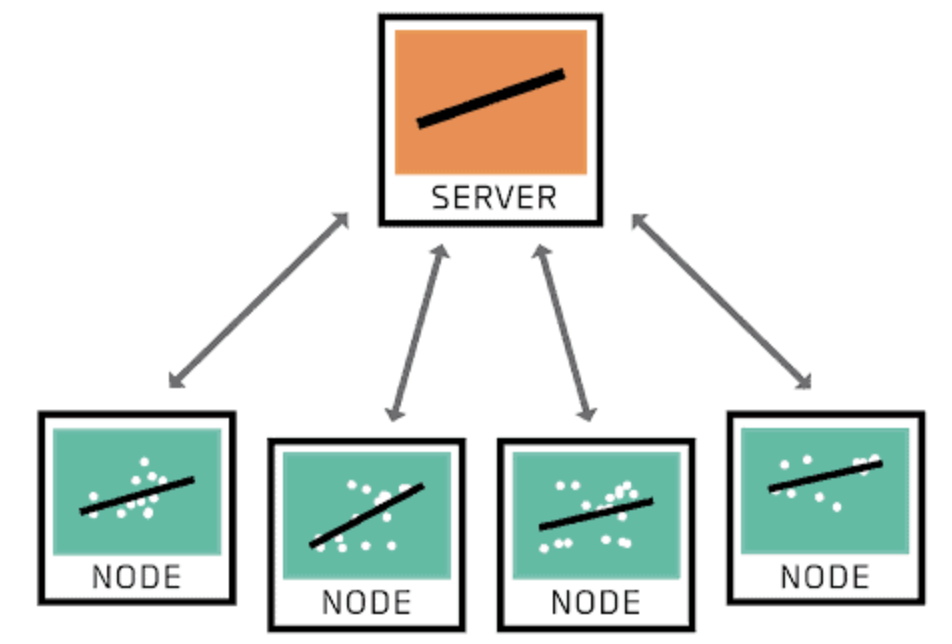
\includegraphics[width=1\textwidth]{images/fl_view}
\end{figure}
\end{column}
\begin{column}{0.65\textwidth}
\textbf{现有联邦学习框架中的问题:}
\begin{itemize}
	\item \textbf{\alert{对于客户端的激励通常被大多数联邦学习框架所忽视。}}激励是指增加客户参加训练后的奖励或收益,使得他们能够更加积极地贡献数据参与训练;
	\item \textbf{\alert{恶意参与者试图破坏联邦学习的全局模型。}}联邦学习通常容易受到敌对客户的操纵,尤其是关于模型和数据投毒攻击,即恶意参与者在训练集中引入大量带有修改标签的数据样本,导致全局模型的错误分类。
	\item \textbf{\alert{私人数据仍然可以通过从参数更新中推断信息来泄露。}}因此,针对中毒攻击的最佳安全策略还应该通过推理提供针对隐私泄露的保护。
\end{itemize}
\end{column}
\end{columns}
\end{frame}

\begin{frame}{1.2 Contributions}{\empty}
\begin{itemize}
\item \textbf{提出了一种基于联合差分隐私的联邦学习框架,可限制攻击者的影响并提供严格的隐私保证。}
\item \textbf{提出了两种基于真实客户端数据的博弈论机制来选择参与的客户端进行训练。}
\item \textbf{对于提出机制进行理论证明和分析。客户端选择机制满足博弈论属性,并且对客户端的策略操纵具有鲁棒性。}
\item \textbf{进行了关于所设计机制的基本原理实验。使用真实世界数据集进行实验,证明了所提出的联邦学习方案的实际有效性。}
\end{itemize}
\end{frame}

\section{Preliminaries}

\begin{frame}{2.1 Game Theory}{\empty}
\begin{columns}
\begin{column}{0.5\textwidth}
博弈论,又称为对策论(Game Theory)、赛局理论等,既是现代数学的一个新分支,也是运筹学的一个重要学科。 博弈论主要研究公式化了的激励结构间的相互作用,是研究具有斗争或竞争性质现象的数学理论和方法。 博弈论考虑游戏中的个体的预测行为和实际行为,并研究它们的优化策略。
\textbf{在联邦学习中,服务器需要招募一些客户端来执行训练任务。但是,由于每个客户端的数据集和计算能力不同,他们参与训练的精力和时间成本等也各不相同。}
\end{column}
\begin{column}{0.5\textwidth}
在文本中:

\textbf{我们的框架将客户选择过程视为拍卖游戏,客户提交他们的成本 $c_i$ 作为出价,服务器根据其预算$B$决定赢家和付款$p_i$。如果服务器选择了客户,则其效用为$u_i = p_i \text{-} c_i$,否则 $u_i = 0$。}

假定客户是理性利己的,每个客户只关心自己的效用并试图最大化它(尽管有可能得到虚假信息)。服务器被激励以其有限的预算 $B$ 吸引尽可能多的参与客户。
\end{column}
\end{columns}
\end{frame}

\begin{frame}{2.2 Definitions}{\empty}
具体来说,客户选择机制应该满足以下博弈论定义:
\begin{definition}[Dominant-strategy truthful]
 A client selection mechanism $\mathcal{M}$ is dominant-strategy truthful if, for every client, truthfully reporting his cost $c_i$ is a dominant strategy. That is, given $c_i$ and all possible $c_i^{\prime} \in \mathbb{R}$ :
$$
u_i\left(c_i, c_{-i}\right) \geq u_i\left(c_i^{\prime}, c_{-i}\right),
$$
where $c_{-i}$ represents the strategy profile of clients except for the $i$ th component, $c=\left(c_i, c_{-i}\right)$.
\end{definition}
真实意味着没有客户可以通过歪曲数据来提高他们的效用,这是开发博弈论解决方案的一个重要属性。
\end{frame}

\begin{frame}{2.2 Definitions}{\empty}
\begin{definition}[Individual rationality]
$\mathrm{A}$ mechanism $\mathcal{M}$ is individual rational for each client if the clients gain nonnegative utility by participating in $\mathcal{M}$.
$$
u_i=p_i-c_i \geq 0 .
$$
\end{definition}
个人理性保证了每个客户的基本效用。如果参与一种机制可能导致负效用,客户可能会完全拒绝参与。
\begin{definition}[Budget balance] A client selection mechanism $\mathcal{M}$ is budget-balanced if the total amount paid by the server does not exceed its budget. Formally, given $m$ selected clients, each receives a payment $p_i$, then
$$
\sum_{i=1}^m p_i \leq B
$$
\end{definition}
最后,从服务器的角度来看,其总支出必须保持在其预定义的预算范围内。
\end{frame}


\section{Methodology}

\begin{frame}{3.1 Overview of the mechanism}{\empty}
\centering
\vspace{0.5em}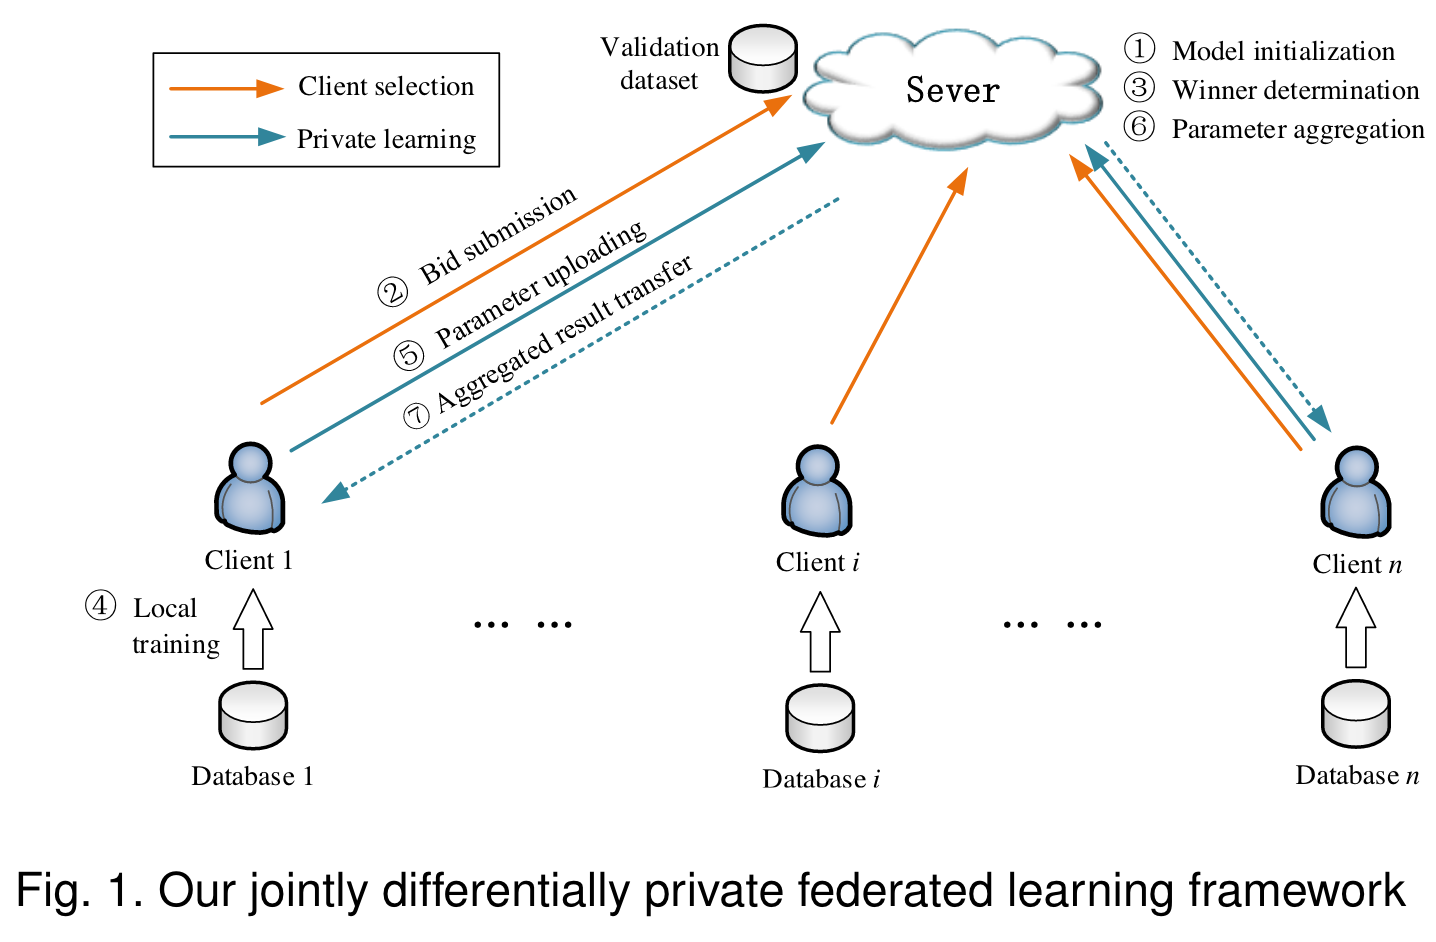
\includegraphics[width=0.8\textwidth]{images/overview}
\end{frame}

\begin{frame}{3.2 Alogrithm 1 - Step\textcircled{3} Winner Determination}{\empty}
\begin{columns}
\begin{column}{0.6\textwidth}
\vspace{0.5em}
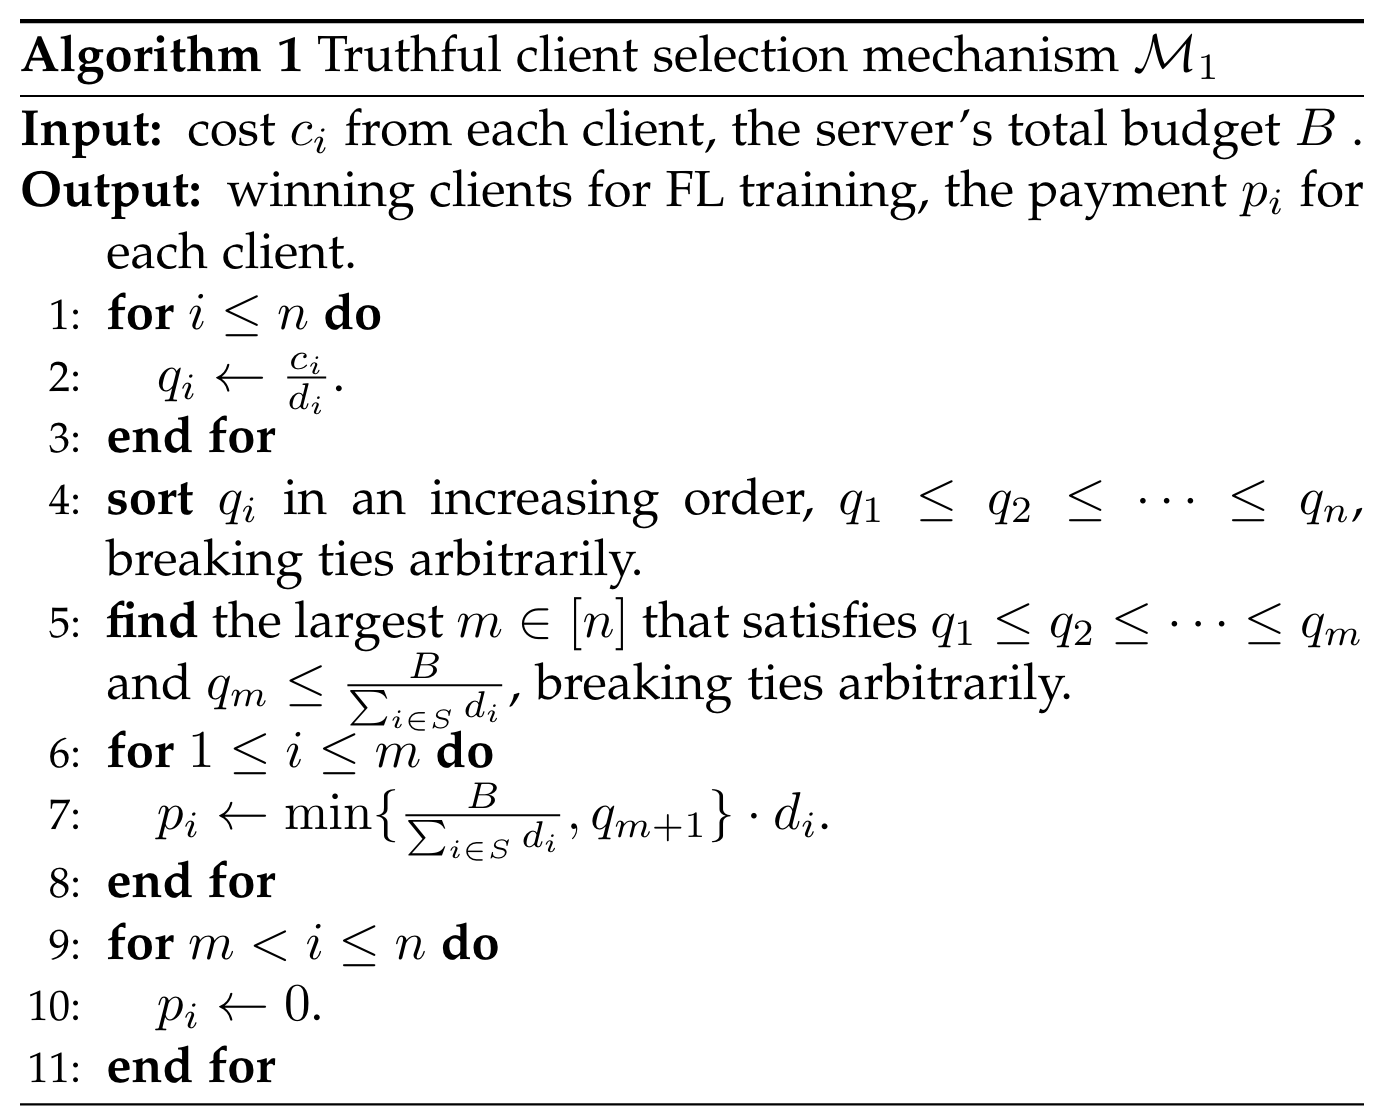
\includegraphics[width=1\textwidth]{images/algo1}
\end{column}
\begin{column}{0.4\textwidth}
$c_i$:训练成本(能源消耗、通信成本和训练数据集的估值来评估成本)\\
$d_i$:数据量\\
$q_i$:单位数据消耗\\
$\frac{B}{\sum_{i \in S} d_i}$:平均单位数据消耗\\
$p_i$:选择该模型需要的支出
\end{column}
\end{columns}
\end{frame}

\begin{frame}{3.2 Alogrithm 2 - Step\textcircled{3} Winner Determination}{\empty}
\begin{columns}
\begin{column}{0.5\textwidth}
\vspace{0.5em}
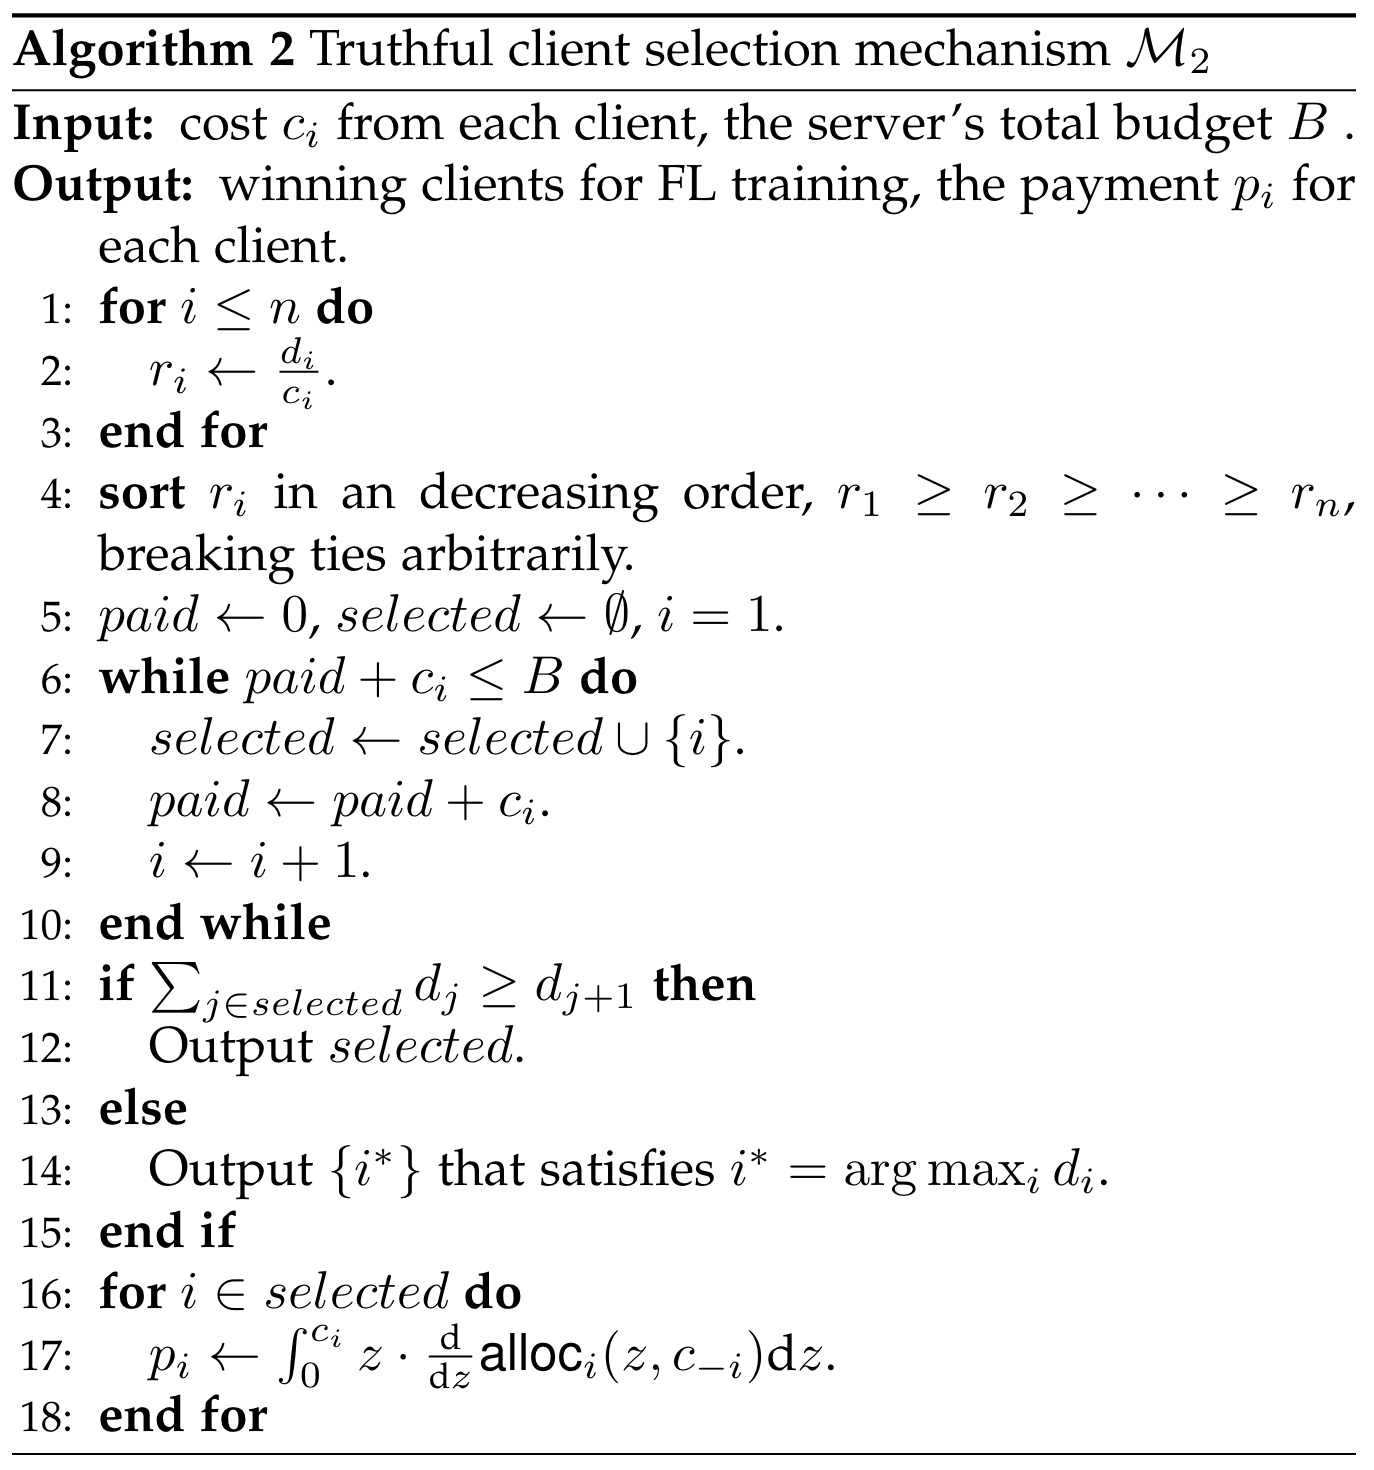
\includegraphics[width=1\textwidth]{images/algo2}
\end{column}
\begin{column}{0.5\textwidth}
\textbf{Knapsack Problems:}
$$
\begin{aligned}
& \max \sum_{i=1}^n x_i \cdot d_i, \\
\text { s.t. } & \sum_{i=1}^n x_i \cdot c_i \leq B, \forall i, x_i \in\{0,1\} .
\end{aligned}
$$
是典型的 0/1 背包问题,其中:\\
$d_i$ 代表每个客户的个性化权重值\\
$c_i$ 是相应的消耗\\
$x_i$是带不带它,取值为0或1\\

$r_i$:ranking,其实就是按效率的排序\\
$p_i$:选择该模型需要的支出
\end{column}
\end{columns}
\end{frame}

\begin{frame}{3.2 Review}{\empty}
\centering
\vspace{0.5em}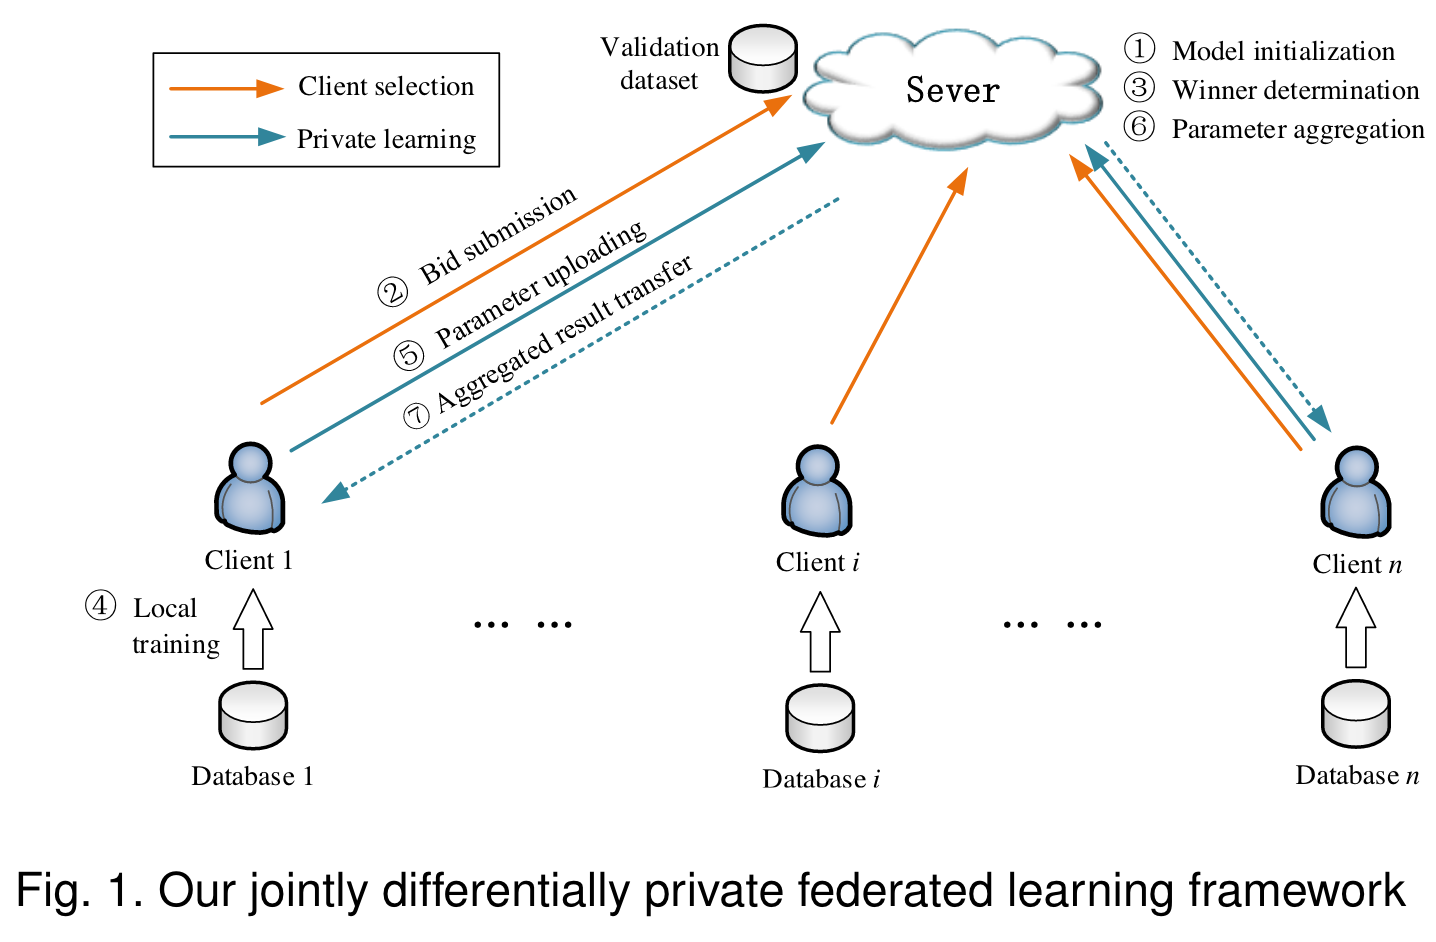
\includegraphics[width=0.8\textwidth]{images/overview}
\end{frame}

\begin{frame}{3.3 Alogrithm 3 - Step\textcircled{5} Parameter Uploading}{\empty}
\begin{columns}
\begin{column}{0.6\textwidth}
\vspace{0.5em}
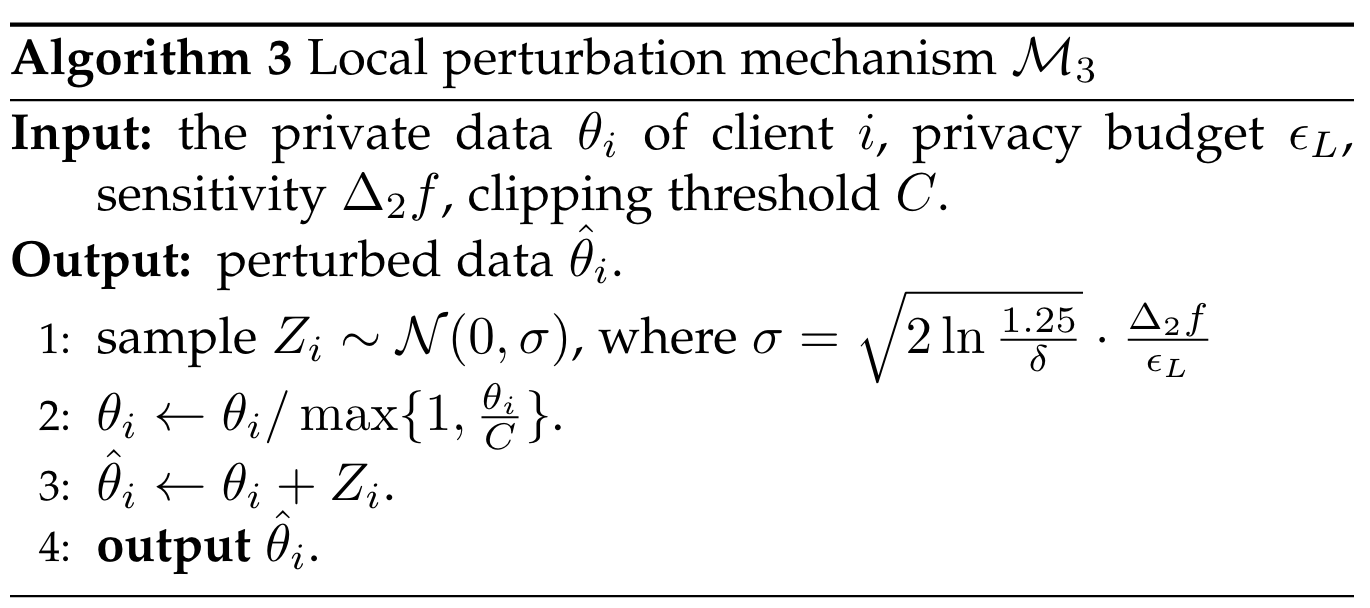
\includegraphics[width=1\textwidth]{images/algo3}
\end{column}
\begin{column}{0.4\textwidth}
DP-SGD\\
$\theta_i$:需要扰动的参数\\
$Z_i$:高斯噪声\\
$C$:梯度范数阈值\\
$p_i$:选择该模型需要的支出\\
$\epsilon$:隐私预算\\
$\delta$:松弛系数
\end{column}
\end{columns}
\end{frame}

\begin{frame}{3.4 Alogrithm 4 - Step\textcircled{6} Parameter Aggregation}{\empty}
\begin{columns}
\begin{column}{0.6\textwidth}
\vspace{0.5em}
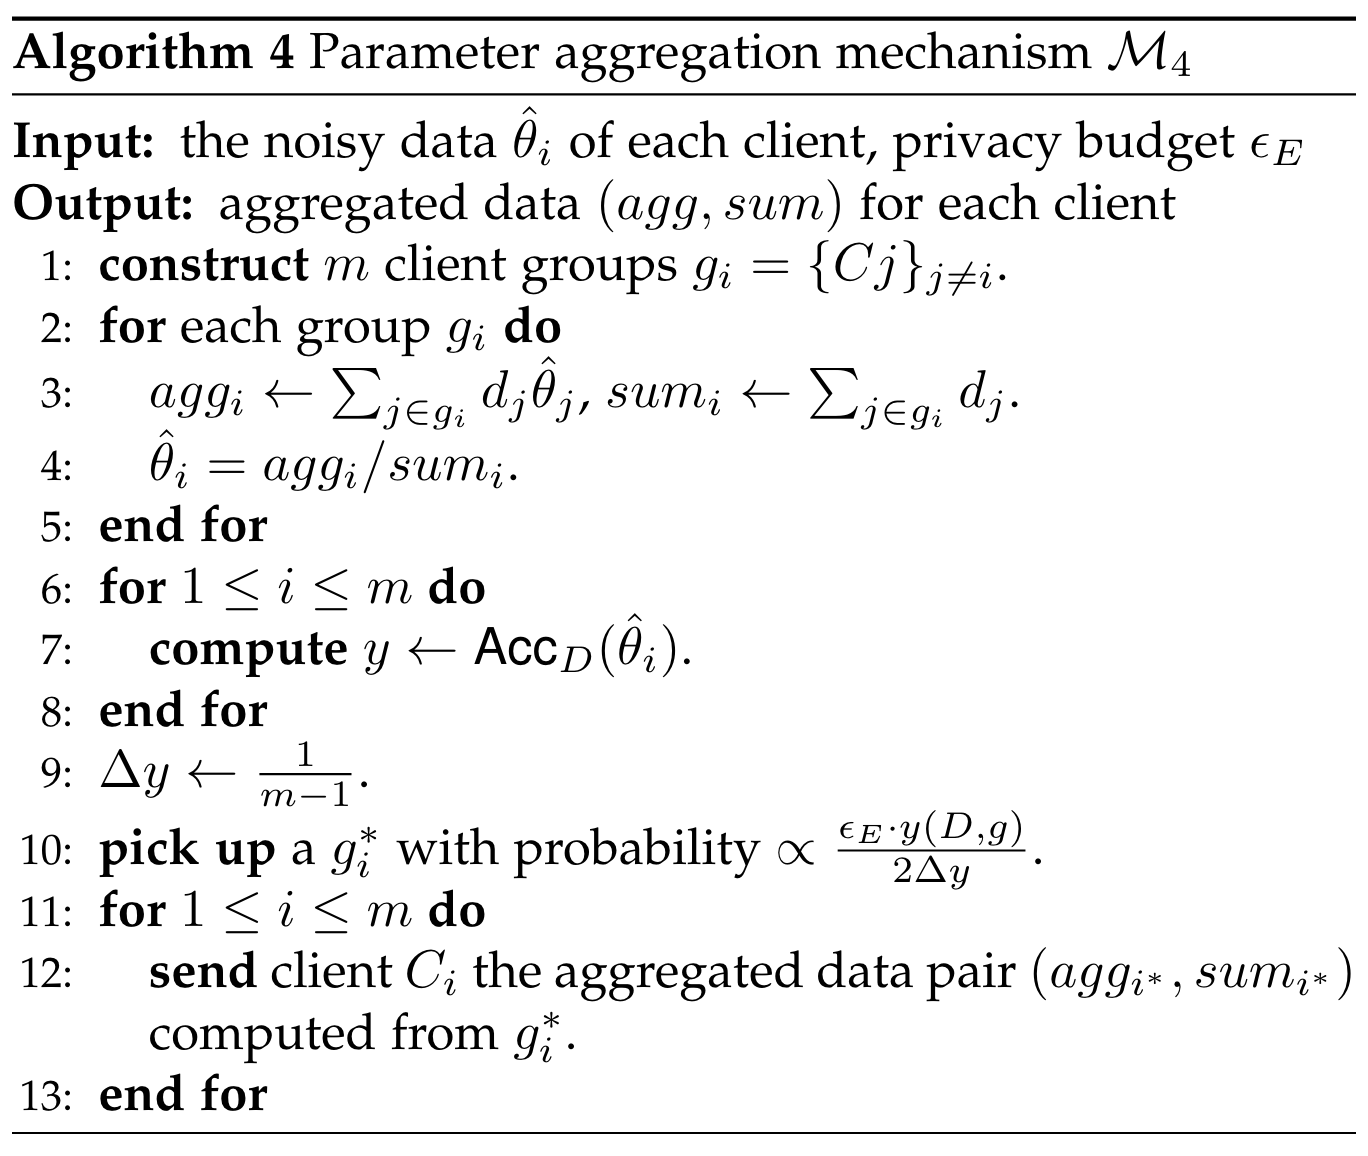
\includegraphics[width=1\textwidth]{images/algo4}
\end{column}
\begin{column}{0.4\textwidth}

$$
\theta=\sum_{i=1}^m d_i \hat{\theta}_i / \sum_{i=1}^m d_i
$$
\\
$g_i$:客户端模型组合,总数其实是 $C_{m}^{m-1}=m$\\
$agg_i$:每组合模型个性化权重值与参数乘积的累和\\
$sum_i$:每组合模型个性化权重值的累和\\
$\hat{\theta_i}$:每组合模型数据量的累和\\
$ACC_D$:得分函数(来自每个客户端组的聚合参数的优秀程度)\\
$\Delta y$:评分函数的灵敏度\\
$g^*_i$:以概率选出的客户端模型组合
\end{column}
\end{columns}
\end{frame}

\begin{frame}{3.5 Alogrithm 5 - Step\textcircled{7} Parameter Result Transfer}{\empty}
\begin{columns}
\begin{column}{0.5\textwidth}
\vspace{0.5em}
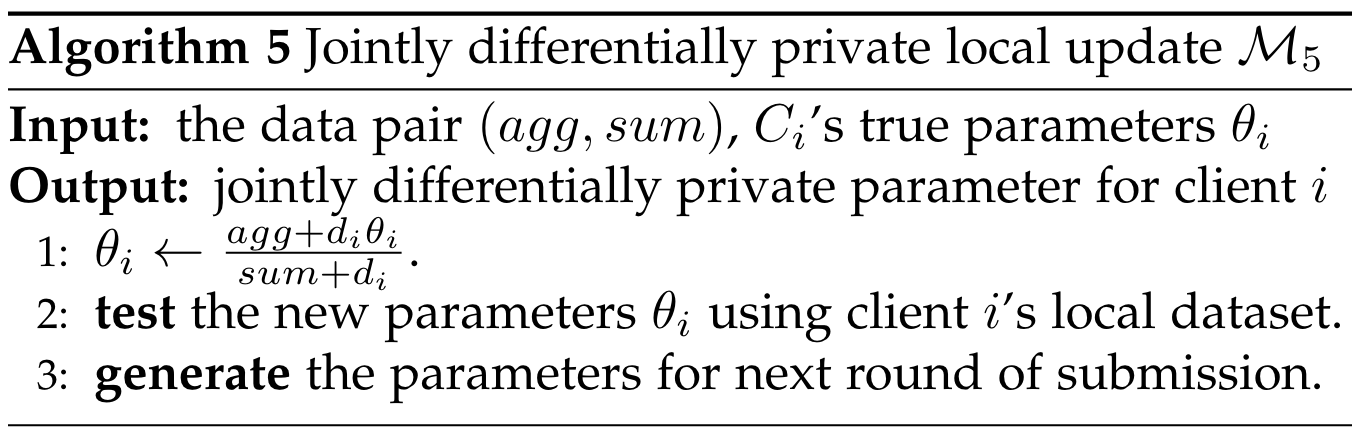
\includegraphics[width=1\textwidth]{images/algo5}
\end{column}
\begin{column}{0.5\textwidth}
$agg_i$:每组合模型个性化权重值与参数乘积的累和\\
$sum_i$:每组合模型个性化权重值的累和\\
$d_i$ 代表每个客户的个性化权重值\\
$\theta_i$:本地参数(没扰动)\\
\end{column}
\end{columns}
\end{frame}






\section{Conclusions}

\begin{frame}{Conclusions}


\begin{itemize}
    \item 在本文中,提出了一个强大的联邦学习框架,解决了激励客户参与联邦学习的实际问题。
    \item 其次,提出了两种新颖的博弈论机制,将客户选择制定为拍卖博弈。客户将他们的成本报告为出价,服务器使用不同的支付策略来最大化其目标。整体框架是联合差分隐私的,这限制了敌对客户的影响。
    \item 此外,我们还对真实世界的数据集进行了模拟,以验证框架的性能。
    \item 结果表明,在我们的方案下,敌对客户对全局模型的准确性几乎没有影响。
  \end{itemize}
  
\end{frame}



\backmatter

\end{document}
